\section{The Big Idea}
We propose the following offline \textbf{symmetry breaking technique}: 
 \begin{wrapfigure}{r}{0.25\columnwidth}
       \vspace{2em}
		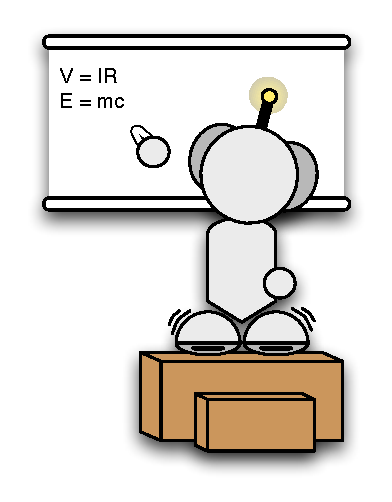
\includegraphics[width=0.25\columnwidth, trim=10mm 10mm 10mm 10mm]{diagrams/robot_whiteboard.pdf}
 \end{wrapfigure}
\begin{enumerate}
\item{Decompose the grid map into a set of empty rectangular rooms.}
\item{Prune all tiles not on the perimeter of an empty room.}
\item{Connect tiles on opposite sides of the perimeter.}
\end{enumerate}
\vspace{1em}
Sometimes a tile which has been pruned is later required; for example as a start
or goal location. 
To handle such cases we use an \textbf{online re-insertion} procedure.
Figure \ref{fig:splash} shows a concrete example.
%by temporarily re-inserting the 
%required tile back into the grid map for the duration of the search.

\begin{figure}[t]
\hspace{0.35in}
\begin{minipage}{17in}
\label{fig:splash}
\begin{center}
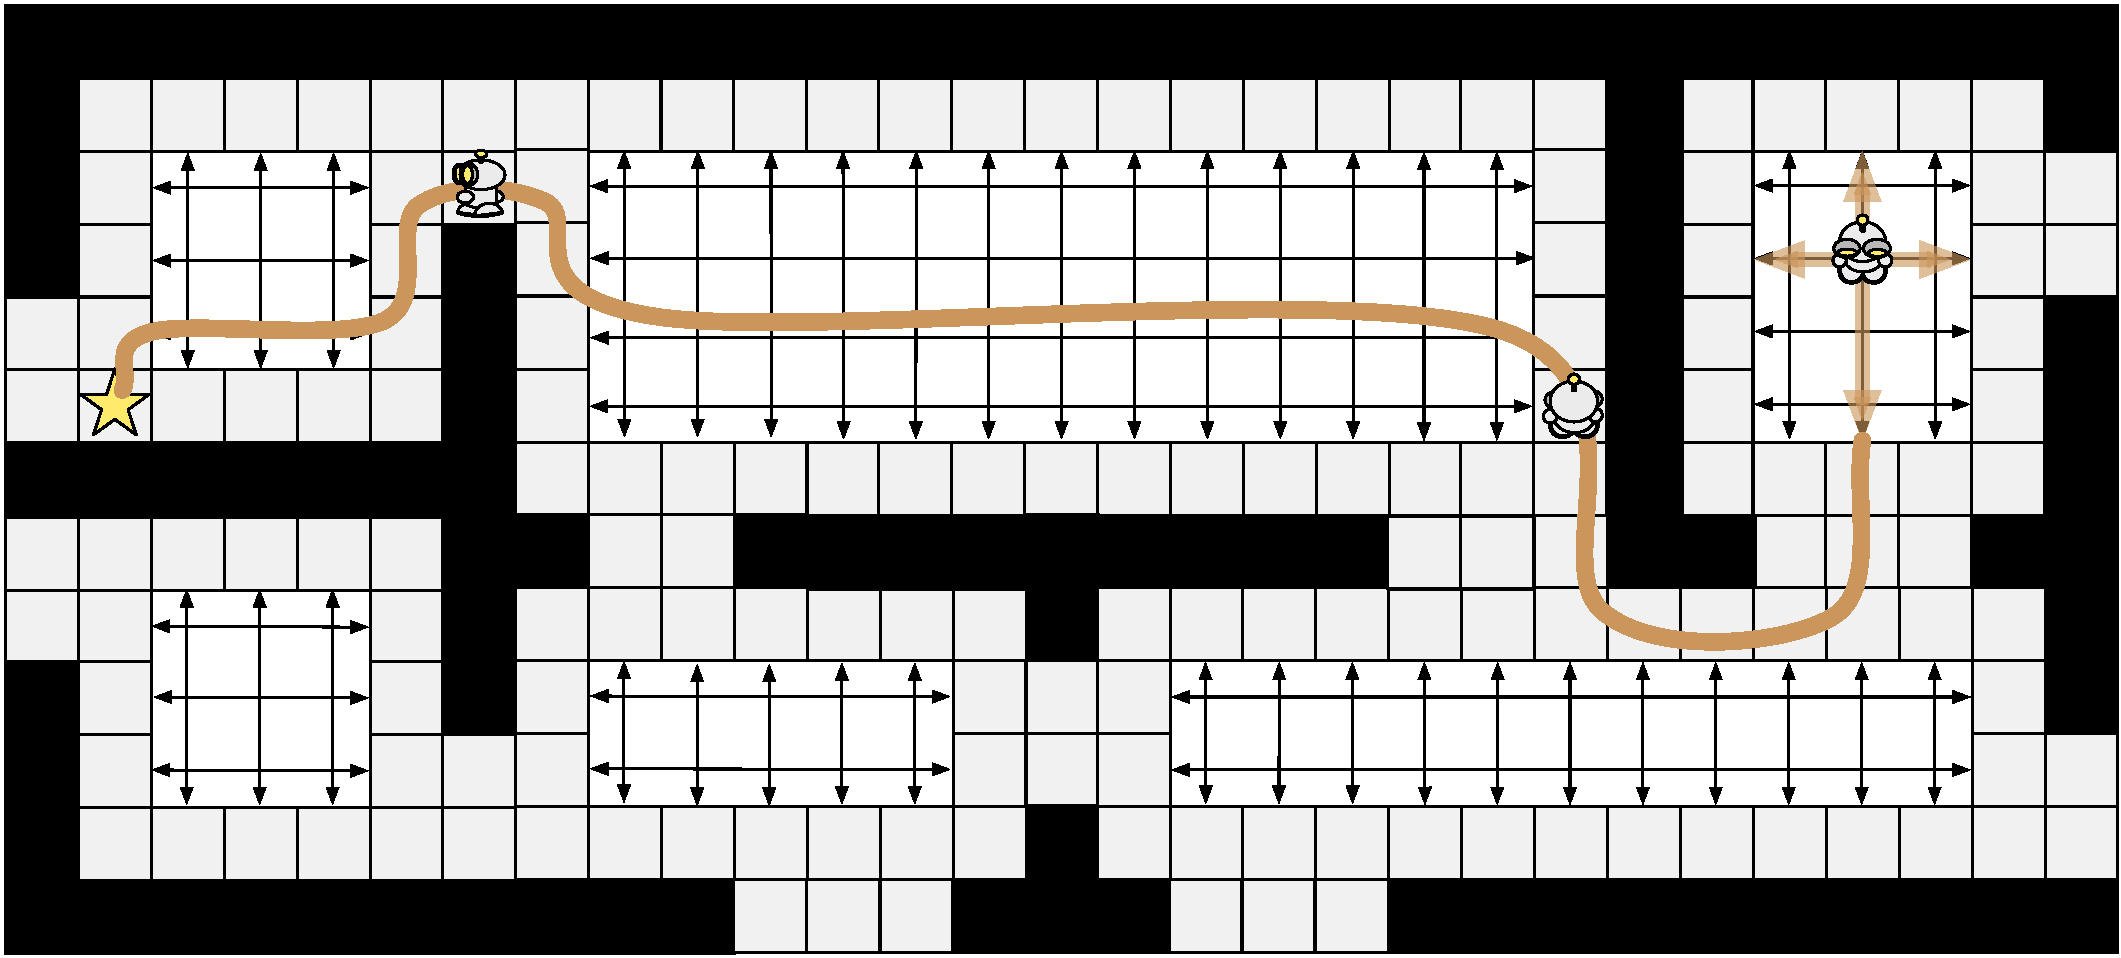
\includegraphics[width=17in]{diagrams/robot_map.pdf}
\caption{We speed up search by decomposing a 4-connected map into empty rectangular
rooms which can be traversed without visiting any tiles from their interior.
This method is both fast and provably optimal.}
\end{center}
\end{minipage}
\vspace{1em}
\end{figure}

\pagebreak
